\documentclass[border=0.2cm]{standalone}
\usepackage{tikz}
\usepackage{amsmath,amssymb}


\usetikzlibrary{chains,fit, shapes,arrows, automata, backgrounds}

\tikzset{%
  block/.style    = {draw, thick, rectangle, minimum height = 1cm,
    minimum width = 1cm, node distance=2cm, fill=blue!10},
  var/.style  = {draw, thick, circle, minimum height = 1cm,
      minimum width = 1cm, node distance=2cm, fill=red!20},
  obs/.style = {draw, minimum size= 0.6cm, node distance=-0.15mm, fill=white},
  roundtangle/.style = {draw, rounded corners=0.5cm, fill=gray!20}
}
\tikzstyle{arrow} = [draw, thick, -latex']
\tikzstyle{line} = [draw]

\begin{document}
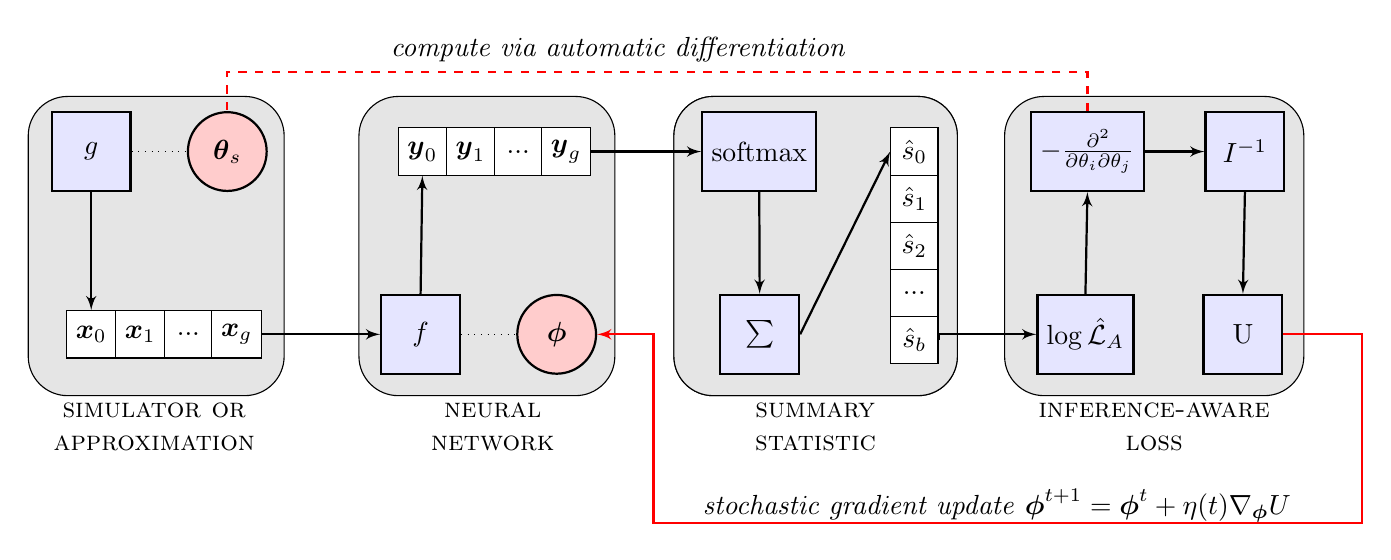
\begin{tikzpicture}[start chain=1 going right,
                    start chain=2 going right,
                    start chain=3 going below,
                    node distance=-0.15mm]

\draw
  node [block] (g) {$g$}
  node [var, right=0.7cm of g] (theta) {$\boldsymbol{\theta}_s$}
;

  \node [on chain=1,obs, below=1.5cm of g] (x_0) {$\boldsymbol{x}_0$};
  \node [on chain=1,obs] (x_1) {$\boldsymbol{x}_1$};
  \node [on chain=1,obs] {...};
  \node [on chain=1,obs] (x_g) {$\boldsymbol{x}_g$};

  \node [on chain=2,obs, right=1.65cm of theta] (y_0) {$\boldsymbol{y}_0$};
  \node [on chain=2,obs] (y_1) {$\boldsymbol{y}_1$};
  \node [on chain=2,obs] {...};
  \node [on chain=2,obs] (y_g) {$\boldsymbol{y}_g$};

  \draw
  node [block, right=1.5cm of x_g] (f) {$f$}
  node [var, right=0.7cm of f] (phi) {$\boldsymbol{\phi}$}

  ;

  \draw
  node [block, right=1.4cm of y_g] (softmax) {softmax}
  node [block, right=1.55cm of phi] (sum) {$\sum$}
  ;

  \node [on chain=3,obs, right=3.8cm of y_g] (s_0) {$\hat{s}_0$};
  \node [on chain=3,obs] (s_1) {$\hat{s}_1$};
  \node [on chain=3,obs] (s_2) {$\hat{s}_{2}$};
  \node [on chain=3,obs] {...};
  \node [on chain=3,obs] (s_b) {$\hat{s}_b$};

  \draw
  node [block, right=3.0cm of sum] (L) {$\log \hat{\mathcal{L}}_A$}
  node [block, right=2.7cm of softmax] (der) {$- \frac{\partial^2}{\partial {\theta_i} \partial {\theta_j}}$}
  node [block, right of=L] (U) {U}
  node [block, right of=der] (inv_hess) {$I^{-1}$}
  ;


  \draw [dashed, thick, red] (der.north) -- ++(0,+0.5cm) -| (theta.north);
  \draw [thick, red, -latex'] (U.east) -| ++(1cm,0) |- ++(0,-2.4cm) --
   ++(-9.0cm,0) -- ++(0,2.4cm) --  (phi.east);

  \draw [dotted] (g.east) -- (theta.west);
  \draw [dotted] (f.east) -- (phi.west);

  \draw [arrow] (g.south) -| (x_0.north);
  \draw [arrow] (x_g.east) -- (f.west);
  \draw [arrow] (f.north) -- (y_0.south);
  \draw [arrow] (y_g.east) -- (softmax.west);
  \draw [arrow] (softmax.south) -- (sum.north);
  \draw [arrow] (sum.east) to (s_0.west);
  \draw [arrow] (s_b.east) |- (L.west);
  \draw [arrow] (L.north) -- (der.south);
  \draw [arrow] (der.east) -- (inv_hess.west);
  \draw [arrow] (inv_hess.south) -- (U.north);


  \node [align=center] at (0.8cm,-3.5cm) {\textsc{simulator or} \\  \textsc{approximation}};
  \node [align=center] at (5.1cm,-3.5cm) {\textsc{neural} \\  \textsc{network}};
  \node [align=center] at (9.2cm,-3.5cm) {\textsc{summary} \\  \textsc{statistic}};
  \node [align=center] at (13.5cm,-3.5cm) {\textsc{inference-aware} \\  \textsc{loss}};

  \node [align=center] at (6.7cm,1.3cm) {\textit{compute via automatic differentiation}};
  \node [align=center] at (11.5cm,-4.5cm) {\textit{stochastic gradient update} $\boldsymbol{\phi}^{t+1}= \boldsymbol{\phi}^{t}+\eta(t)\nabla_{\boldsymbol{\phi}}U$};

  \begin{pgfonlayer}{background}
  \draw[roundtangle]
  (-0.8cm,-3.1cm) rectangle ++(3.25cm,3.8cm);
  \draw[roundtangle]
  (3.4cm,-3.1cm) rectangle ++(3.25cm,3.8cm);
  \draw[roundtangle]
  (7.4cm,-3.1cm) rectangle ++(3.6cm,3.8cm);
  \draw[roundtangle]
  (7.4cm,-3.1cm) rectangle ++(3.6cm,3.8cm);
  \draw[roundtangle]
  (11.6cm,-3.1cm) rectangle ++(3.8cm,3.8cm);
  \end{pgfonlayer}

\end{tikzpicture}
\end{document}
